%%%%%%%%%%%%%%%%%%%%%%%%%%%%%%%%%%%%%%%%%%%%%%%%%%%%%%%%%%%%%%%
%
% Welcome to Overleaf --- just edit your LaTeX on the left,
% and we'll compile it for you on the right. If you open the
% 'Share' menu, you can invite other users to edit at the same
% time. See www.overleaf.com/learn for more info. Enjoy!
%
%%%%%%%%%%%%%%%%%%%%%%%%%%%%%%%%%%%%%%%%%%%%%%%%%%%%%%%%%%%%%%%


% Inbuilt themes in beamer
\documentclass{beamer}

% Theme choice:
\usetheme{CambridgeUS}

% Title page details: 

\usepackage{polynom}
\usepackage{amssymb}
\usepackage{amsmath}

\usepackage{bm}
\usepackage[misc]{ifsym}

\usepackage{longtable}
\usepackage{enumitem}
\usepackage{mathtools}
\usepackage[applemac]{inputenc}
\usepackage{tikz}
\usepackage{listings}
    \usepackage{color}                                            %%
    \usepackage{array}                                            %%
    \usepackage{longtable}                                        %%
    \usepackage{calc}                                             %%
    \usepackage{multirow}                                         %%
    \usepackage{hhline}                                           %%
    \usepackage{ifthen}                                           %%
  
\usepackage{lscape}     
\usepackage{tfrupee}
\usepackage{parskip}

\DeclareMathOperator*{\Res}{Res}
\DeclareMathOperator*{\equals}{=}
\DeclareMathOperator*{\pipe}{|}

\hyphenation{op-tical net-works semi-conduc-tor}
\def\inputGnumericTable{}  
\graphicspath{{./images/}}


\begin{document}
\newcommand{\bfr}[2]{\section{#1} \begin{frame}{#1} #2 \end{frame}}

	\title{Assignment 9}
		\author{ Abhay Shankar K : CS21BTECH11001}
\date{}
	\begin{frame}
    		\titlepage 
	\end{frame}

	\begin{frame}{Outline}
    		\tableofcontents
	\end{frame}

	\providecommand{\brak}[1]{\ensuremath{\left(#1\right)}}
	\providecommand{\sbrak}[1]{\ensuremath{\left[#1\right]}}
	\providecommand{\cbrak}[1]{\ensuremath{\left\{#1\right\}}}
	\providecommand{\req}{\textbf{Required :}}
	\providecommand{\rpr}[2]{\ensuremath{P_{#1}\left(#2\right)}} %random variable notation
	\providecommand{\spr}[1]{\ensuremath{P\left(#1\right)}} %simple notation
	\providecommand{\cpr}[2]{\ensuremath{\spr{#1 \pipe #2}}} %conditional probability
	\newcommand*{\permcomb}[4][0mu]{{{}^{#3}\mkern#1#2_{#4}}}
	\newcommand*{\perm}[1][-3mu]{\permcomb[#1]{P}}
	\newcommand*{\comb}[1][-1mu]{\permcomb[#1]{C}}
	\newcommand{\abs}[1]{\left| #1 \right|}
	\newcommand{\pow}[2]{\ensuremath{#1^{#2}}}
	\newcommand{\e}[1]{\pow{e}{#1}}
	
	\providecommand{\pdf}[2]{\ensuremath{f_{#2}\left(#1\right)}}
	\providecommand{\cdf}[2]{\ensuremath{F_{#2}\left(#1\right)}}
	
	\bfr{Question}{
	
	Express the density \pdf{y}{y} of the random variable $y = g \brak{x}$ in terms of \pdf{x}{x} if :
	\begin{enumerate}[label = \brak{\textbf{\roman*}}]
	
		\item $g \brak{x} = \abs{x}$
		
		\item $g \brak{x} = \e{-x} U\brak{x}$ where U \brak{x} is the Uniform Distribution, say over the interval \sbrak{-1, 1}.		
	\end{enumerate}
	
	}
	
	\bfr{Solution : \brak{\textbf{\textrm{i}}}}{
	
		Clearly, \pdf{0}{y} = \pdf{0}{x}. For nonzero $x$ :
		 
		We know 
		\begin{align} 
			\cdf{y_1}{y} &= \spr{g \brak{x} \leq g \brak{x_1}} \nonumber \\
			&= \spr{\abs{x} \leq \abs{x_1}} \nonumber\\
			&= \spr{-\abs{x_1} \leq x \leq \abs{x_1}} \nonumber\\
			&= \brak{\cdf{x_1}{x} - \cdf{-x_1}{x}} \times sgn\brak{x_1} \nonumber \\
			\nonumber\\
			\therefore \cdf{y}{y} &= \brak{\cdf{x}{x} - \cdf{-x}{x}} sgn\brak{x}
				\label{cdf_1}
		\end{align}
		
		Assuming \pdf{x}{x} is a normal distribution, clearly the normalization factor is $0.5$. Differentiating and normalizing ~\eqref{cdf_1},
		\begin{align}
			\pdf{y}{y} = \frac{1}{\sigma \sqrt{2 \pi}} \times \e{\frac{x^2}{2 \sigma^2}} \label{norm_i}
		\end{align}
}

\bfr{Solution : \brak{\textbf{\textrm{ii}}}}{
	
		We know 
		\begin{align} 
			\cdf{y_1}{y} &= \spr{g \brak{x} \leq g \brak{x_1}} \nonumber \\
			&= \spr{\e{-x} \leq \e{-x_1}} \nonumber\\
			&= \spr{x \geq x_1} \nonumber\\
			&= 1 - \spr{x \leq x_1} + \rpr{x}{x_1} \nonumber\\
			&= 1 - \cdf{x_1}{x} \nonumber \\
			\nonumber\\
			\therefore \cdf{y}{y} &= 1 - \cdf{\frac{-\ln{y}}{U \brak{x}}}{x}
				\label{cdf_2}
		\end{align}
		
		Assuming \pdf{x}{x} is a normal distribution and $\sigma = 0.3$, the normalization constant is $0.1618$. Differentiating and normalizing~\eqref{cdf_2},
		\begin{align}
			\pdf{y}{y} = \brak{1 +  \frac{4}{\sigma \sqrt{2 \pi}} \e{x - \frac{x^2}{2 \sigma^2}} } \times 0.1618 \label{norm_ii}
		\end{align}

}

\bfr{Result}{
	\begin{enumerate}[label = \brak{\textbf{\roman*}}]
	
		\item $y = \abs{x} \implies \pdf{y}{y} = \pdf{y}{y} = \frac{1}{\sigma \sqrt{2 \pi}} \times \e{\frac{x^2}{2 \sigma^2}} \rightarrow ~\eqref{norm_i}$
		
		\item $y = \e{-x} U\brak{x} \implies \pdf{y}{y} = \brak{1 +  \frac{4}{\sigma \sqrt{2 \pi}} \e{x - \frac{x^2}{2 \sigma^2}} } \times 0.1618 \rightarrow ~\eqref{norm_ii}$		
	\end{enumerate}

}

\bfr{Graph}{
	Assuming : $\sigma = 0.3$
		
	\begin{figure}[h!]
		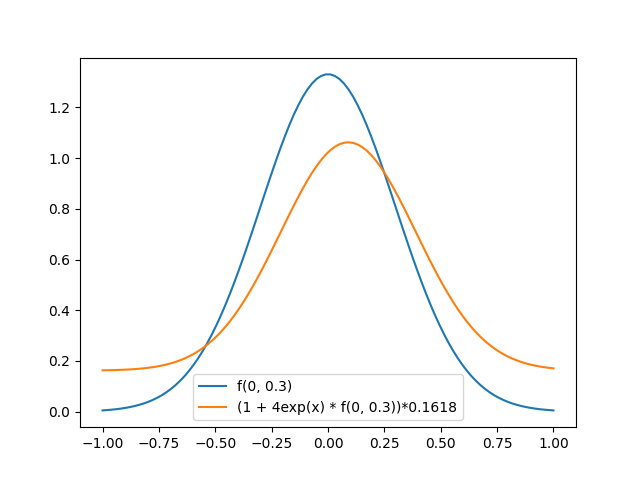
\includegraphics[scale = 0.4]{assig9}
	\end{figure}
	
	}
							
\end{document}
	
	

	
	
	
	